\chapter{Geometria (4º Bimestre)}

\section{Teorema de Tales}

De acordo com a Wikipedia, ``o teorema de Tales afirma que quando duas retas
transversais cortam um feixe de retas paralelas, as medidas dos segmentos
delimitados nas transversais são proporcionais''.

Por exemplo, na figura a seguir, consideramos um triângulo $ABC$ e traçamos três
retas (vermelha, verde e azul) paralelas ao lado $AB$. Obtemos três triângulos
${A_1B_1C_1}$, ${A_2B_2C_2}$, ${A_3B_3C_3}$ semelhantes a $ABC$:

\begin{center}
 \begin{tikzpicture}
   \draw (0,0)node[below left] {$A$} -- (0,4) node[above left] {$B$}
   -- (3,1) node[right] {$C$} -- (0,0)[color=orange];
   \draw (6,-2) -- (3,1) -- (6,2)[dashed];
   \draw (0,0) -- (-3,-1)[dashed];
   \draw (0,4) -- (-3,7)[dashed];

   \draw (-1,7) -- (-1,5)node[above left] {$B_1$} --
   (-1,-0.33333333333333)node[below left] {$A_1$} -- (-1,-3)[red];
   \draw (2,7) -- (2,2)node[above right] {$B_2$} --
   (2,0.66666666666666)node[below right] {$A_2$} -- (2,-3)[green];
   \draw (5,7) -- (5,1.66666666666666)node[above right] {$A_3$}
   -- (5,-1)node[below right] {$B_3$} -- (5,-3)[blue];
   \
 \end{tikzpicture}
\end{center}

e temos:
%%
$$
\frac{CA}{CA_1} = \frac{CB}{CB_1} = \frac{AB}{A_1B_1}
$$
%%
$$
\frac{CA_2}{CA} = \frac{CB_2}{CB} = \frac{A_2B_2}{AB}
$$
%%
$$
\frac{CA}{CA_3} = \frac{CB}{CB_3} = \frac{AB}{A_3B_3}
$$

\subsection*{Exercício 3 (Tales)}

Na figura anterior, utilize os resultados do primeiro capítulo para explicar por
que

\begin{enumerate}
\item $\widehat{BCA} = \widehat{B_3CA_3}$?
\item $\widehat{CA_3B_3} = \widehat{CAB}$ e $\widehat{CB_3A_3} = \widehat{CBA}$?
\item $\widehat{CA_1B_1} = \widehat{CA_2B_2} = \widehat{CAB}$ e
  $\widehat{CB_1A_1} = \widehat{CB_2A_2} = \widehat{CBA}$?
\end{enumerate}

Deduzindo o teorema de Tales.

\subsection*{Exercício 4 (pirâmide de Keops)}

Segundo uma lenda, Tales de Mileto empregou seu teorema para medir a altura da
pirâmide de Keops:

\begin{center}
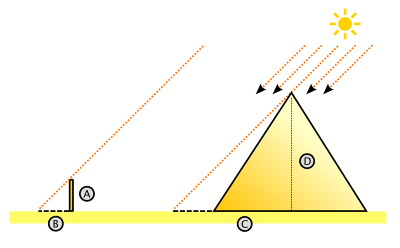
\includegraphics{cheops.png}\\
Fonte: Wikimedia Commons
\end{center}

Determine a altura da pirâmide a partir dessas medidas:

\begin{itemize}
  \item altura da vara: 1.63m.
  \item sombra da vara: 2m.
  \item longitude da base da pirâmide: 230m.
  \item sombra da pirâmide: 65m.
\end{itemize}

\subsection*{Exercício 5}

Neste exercício, considere um segmento unitário sobre uma folha de papel e
queremos construir outra longitude, utilizando somente regra e compasso.

\begin{center}
 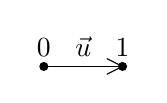
\begin{tikzpicture}
   \draw (0,0)node[above]{$0$} -- (0.5,0)node[above]{$\vec{u}$} -- (1,0)node[above]{$1$};
   \draw (.8,.1) -- (1,0) -- (.8,-.1);
   \draw[fill=black] (0,0) circle(.05);
   \draw[fill=black] (1,0) circle(.05);
 \end{tikzpicture}
\end{center}

Indique como construir os números naturais $0$, $1$, $2$, $3$, \ldots

\begin{center}
 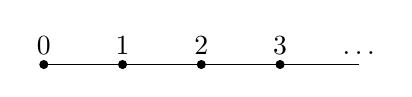
\begin{tikzpicture}
   \draw (0,0)node[above]{$0$} -- (1,0)node[above]{$1$}
   -- (2,0)node[above]{$2$} -- (3,0)node[above]{$3$}
   -- (4,0)node[above]{$\ldots$};
   \draw[fill=black] (0,0) circle(.05);
   \draw[fill=black] (1,0) circle(.05);
   \draw[fill=black] (2,0) circle(.05);
   \draw[fill=black] (3,0) circle(.05);
 \end{tikzpicture}
\end{center}

Indique como construir o eixo ortogonal:

\begin{center}
 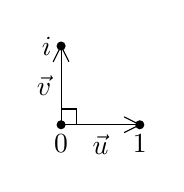
\begin{tikzpicture}
   \draw (0,0)node[below]{$0$} -- (0.5,0)node[below]{$\vec{u}$} -- (1,0)node[below]{$1$};
   \draw (.8,.1) -- (1,0) -- (.8,-.1);
   \draw (0,0) -- (0,0.5)node[left]{$\vec{v}$} -- (0,1)node[left]{$i$};
   \draw (.1,.8) -- (0,1) -- (-.1,.8);
   \draw[fill=black] (0,0) circle(.05);
   \draw[fill=black] (1,0) circle(.05);
   \draw[fill=black] (0,1) circle(.05);
   \draw (0,.2) -- (.2,.2) -- (.2,0);
 \end{tikzpicture}
\end{center}

Agora, consideremos dois inteiros distintos $p, q > 0$. Seja $D$ a reta
(vermelha) passando pelos pontos $(q,0)$ e $(0,1)$. Indique como traçar a reta
(azul) passando por $(p,0)$ e paralela a $D$.

\begin{center}
 \begin{tikzpicture}
   \draw (0,0)node[below]{$0$} -- (0.5,0)node[below]{$\vec{u}$} -- (1,0)node[below]{$1$} -- (8,0);
   \draw (.8,.1) -- (1,0) -- (.8,-.1);
   \draw (0,0) -- (0,0.5)node[left]{$\vec{v}$} -- (0,1)node[left]{$i$} -- (0,5);
   \draw (.1,.8) -- (0,1) -- (-.1,.8);
   \draw[fill=black] (0,0) circle(.05);
   \draw[fill=black] (1,0) circle(.05);
   \draw[fill=black] (0,1) circle(.05);
   \draw (0,.2) -- (.2,.2) -- (.2,0);


   \draw[fill=black] (3,0) circle(.05) node[below]{$q$};
   \draw[fill=black] (7,0) circle(.05) node[below]{$p$};


   \draw[color=red] (-3,2) -- (6,-1);
   \draw[color=blue] (-3,3.333333333333333) -- (7,0);

 \end{tikzpicture}
\end{center}

Qual é o ponto de intersecção da reta azul com o eixo ortogonal? Deduza que
todos os números racionais podem ser construídos com régua e compasso.

\section{Teorema de Pitágoras}

E um triângulo retângulo, os catetos são os dois lados menores e a hipotenusa é
o lado maior. O teorema de Tales diz que em todo triângulo retângulo o quadrado
da hipotenusa é igual a soma dos quadrados dos catetos.

\begin{center}
 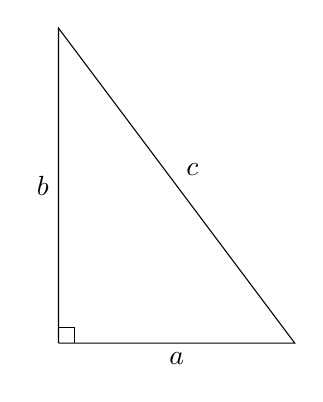
\begin{tikzpicture}
   \draw (0,0) --
   (1.5,0)node[below]{$a$} -- (3,0) --
   (1.5,2)node[above right]{$c$} -- (0,4) --
   (0,2)node[left]{$b$} -- (0,0);
   \draw (0,.2) -- (.2,.2) -- (.2,0);
 \end{tikzpicture}
\end{center}

$$
a^2 + b^2 = c^2
$$

\subsection*{Exercício 6}

Determine as longitude $a$, $b$ e $c$ dos lados de um triângulo retângulo
(figura anterior), se

\begin{enumerate}
\item $a = 12$ e $b = 35$?
\item $b = 56$ e $c = 65$?
\item $a = 11$ e $c = 61$?
\end{enumerate}

\subsection*{Exercício 7}

Considere a figura a seguir:

\begin{center}
 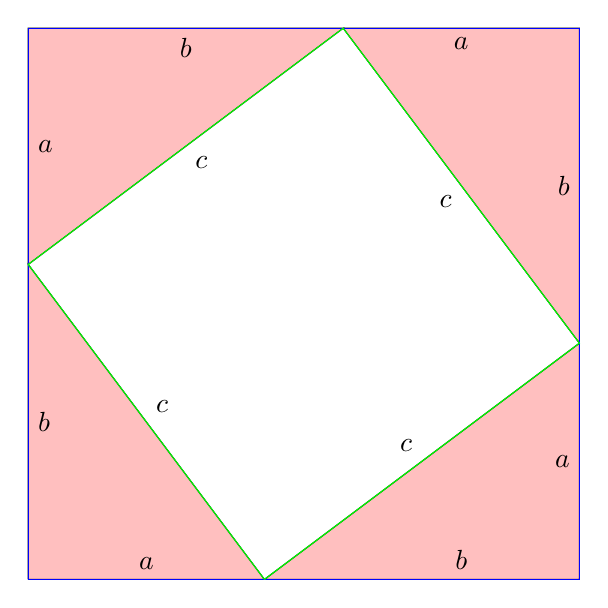
\begin{tikzpicture}

   \draw[color=black,fill=pink]
   (0,0) --
   (1.5,0)node[above]{$a$} -- (3,0) --
   (1.5,2)node[above right]{$c$} -- (0,4) --
   (0,2)node[right]{$b$} -- (0,0);

   \draw[color=black,fill=pink]
   (0,4) --
   (0,5.5)node[right]{$a$} -- (0,7) --
   (2,7)node[below]{$b$} -- (4,7) --
   (2,5.5)node[below right]{$c$} -- (0,4);

   \draw[color=black,fill=pink]
   (4,7) --
   (5.5,7)node[below]{$a$} -- (7,7) --
   (7,5)node[left]{$b$} -- (7,3) --
   (5.5,5)node[below left]{$c$} -- (4,7);

   \draw[color=black,fill=pink]
   (7,3) --
   (7,1.5)node[left]{$a$} -- (7,0) --
   (5.5,0)node[above]{$b$} -- (3,0) --
   (5,1.5)node[above left]{$c$} -- (7,3);

   \draw[color=blue]
   (0,0) -- (7,0) -- (7,7) -- (0,7) -- (0,0);

   \draw[color=green]
   (3,0) -- (7,3) -- (4,7) -- (0,4) -- (3,0);

 \end{tikzpicture}
\end{center}

Expresse em função de $a$, $b$ e $c$:

\begin{itemize}
  \item A área $A$ do quadrado pequeno (verde).
  \item A área $C$ do quadrado grande (azul).
  \item A área $B$ (rosa) que corresponde a quatro triângulos retângulos.
\end{itemize}

Da igualdade $C = A + B$ deduza o teorema de Pitpagoras: $c^2 = a^2 + b^2$.

\subsection*{Exercício 8 (construção da raiz quadrada)}

Suponha que temos uma longitude unitária e outra longitude $x$. Explique como
obtemos a figura a seguir com régua e compasso:

\begin{center}
 \begin{tikzpicture}
   \draw[color=red, dashed] (10,0) arc (0:180:5);
   \draw(1.2,0) -- (1.2,.2) -- (1,.2);

   \draw(0,0) -- (0.5,0)node[below]{$1$} -- (1,0) --
   (5.5,0)node[below]{$x$} -- (10,0);
   \draw(1,0) -- (1,1.5)node[right]{$h$} -- (1,3);
   \draw(1,3) -- (5.5,1.5)node[above right]{$b$} -- (10,0);
   \draw(1,3) -- (.5,1.5)node[above left]{$a$} -- (0,0);

   \draw[color=blue]
   (0,-.5) -- (0,-1) -- (5,-1)node[below]{$c = 1 + x$} -- (10,-1) -- (10, -.5);
 \end{tikzpicture}
\end{center}

O teorema de Tales afirma que o triângulo inscrito no círculo vermelho, de lado
$a$, $b$ e $c$ é retângulo (exercício 6 do primeiro capítulo). Utilize o Teorema
de Pitágoras nesse triângulo e em outros dois para obter a relação $h = \sqrt{x}$.

\subsection*{Exercício 9}

Utilize as técnicas dos exercícios 5 e 8 para construir
$x = \frac{17}{3}$, $p = \sqrt{17}$, $q = \sqrt{3}$, $\sqrt{x}$ e $\frac{p}{q}$.
Verifique geometricamente que
$$
\sqrt{\frac{17}{3}} = \frac{\sqrt{17}}{\sqrt{3}}
$$

\section{Área de polígonos}

\subsection*{Definição}

A soma das longitudes dos lados do polígono se chama perímetro. O tamanho da
região interna do polígono se chama área.

Por exemplo, um retângulo de lados $a$ e $b$ possui perímetro
$a+b+a+b=2{(a+b)}$ e área $a \times b$.

\begin{center}
 \begin{tikzpicture}
   \draw[color=red] (0,0) -- (2,0)node[below]{$a$} --
   (4,0) -- (4,1)node[right]{$b$} --
   (4,2) -- (2,2)node[above]{$a$} --
   (0,2) -- (0,1)node[left]{$b$} --
   (0,0);
 \end{tikzpicture}
\end{center}

\subsection*{Exercício 10 (Quadriláteros)}

\begin{enumerate}
\item
 Qual é o perímetro e a área de um quadrado de lado $a$?

\begin{center}
 \begin{tikzpicture}
   \draw[color=red] (0,0) --
   (2,0) -- (2,1)node[right]{$a$} --
   (2,2) --
   (0,2) --
   (0,0);
 \end{tikzpicture}
\end{center}

\item Seja $a$ e $b$ as longitudes das diagonais de um losango e $c$ a medida
  de um lado. Expresse o perímetro do losango em função de $c$ e
  a área do losango em função de $a$ e $b$ (utilize a área do retângulo azul)?
  
\begin{center}
 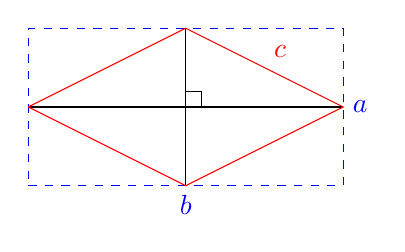
\begin{tikzpicture}
   \draw (2.2,0) -- (2.2,.2) -- (2,.2);
   \draw (0,0) -- (4,0);
   \draw (2,-1) -- (2,1);
   \draw[dashed,color=blue] (0,-1) --
   (2,-1)node[below]{$b$} --
   (4,-1) -- (4,0)node[right]{$a$} -- (4,1) -- (0,1) -- (0,-1);
   \draw[color=red] (0,0) -- (2,-1) -- (4,0) -- (3,.5)node[above right]{$c$} --
   (2,1) -- (0,0);
 \end{tikzpicture}
\end{center}

\item Seja $a$ e $b$ as longitudes de um lado de um paralelogramo e $h$ a
  distância entre os dois lados paralelos de longitude $a$.
  Expresse o perímetro do paralelogramo em função de $a$ e $b$ e
  a área do paralelogramo em função de $a$ e $h$.

\begin{center}
 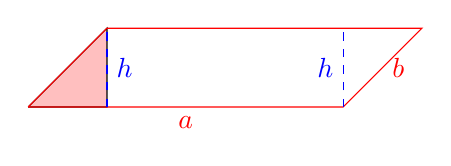
\begin{tikzpicture}
   \draw[color=transparent,fill=pink] (0,0) -- (1,0) -- (1,1) -- (0,0);
   \draw[color=red] (0,0) -- (2,0)node[below]{$a$} --
   (4,0) -- (4.5,.5)node[right]{$b$} -- (5,1) -- (1,1) -- (0,0);
   \draw[dashed,color=blue] (1,0) -- (1,.5)node[right]{$h$} -- (1,1);
   \draw[dashed,color=blue] (4,0) -- (4,.5)node[left]{$h$} -- (4,1);
 \end{tikzpicture}
\end{center}

\item Seja $a$ e $b$ as longitudes dos lados paralelos de um trapezoide e $h$ a
  distância entre os dois lados.
  Expresse a área do trapezoide em função de $a$, $b$ e $h$ (utilize o
  paralelogramo maior formado por duas copias do trapezoide).

\begin{center}
 \begin{tikzpicture}
   \begin{scope}[rotate around={180:(3.75,.5)}]
   \draw[dashed,color=red] (0,0) --
   (4,0) -- (3.5,1) -- (1,1) -- (0,0);
   \end{scope}

   \draw[color=red] (0,0) -- (2,0)node[below]{$a$} --
   (4,0) -- (3.5,1) -- (2.5,1)node[above]{$b$} -- (1,1) -- (0,0);

   \draw[dashed,color=blue] (1,0) -- (1,.5)node[right]{$h$} -- (1,1);
 \end{tikzpicture}
\end{center}

\begin{center}
 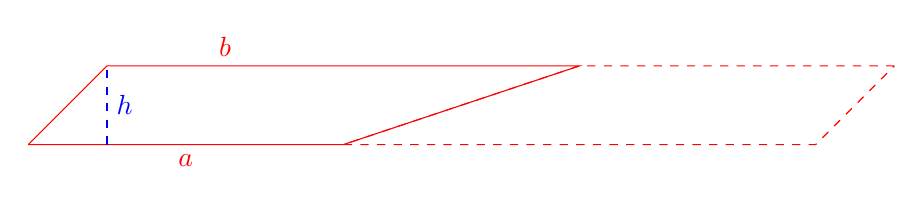
\begin{tikzpicture}
   \begin{scope}[rotate around={180:(5.5,.5)}]
   \draw[dashed,color=red] (0,0) --
   (4,0) -- (7,1) -- (1,1) -- (0,0);
   \end{scope}

   \draw[color=red] (0,0) -- (2,0)node[below]{$a$} --
   (4,0) -- (7,1) -- (2.5,1)node[above]{$b$} -- (1,1) -- (0,0);

   \draw[dashed,color=blue] (1,0) -- (1,.5)node[right]{$h$} -- (1,1);
 \end{tikzpicture}
\end{center}

\end{enumerate}

\subsection*{Exercício 11 (Triângulo)}

\begin{enumerate}
\item Expresse o perímetro de um triângulo de lados $a$, $b$ e $c$.
\item Formule expressões do perímetro para um triângulo isósceles,
  equilátero, rectângulo e isósceles rectângulo.
\item Expresse a área de um triângulo de lado $a$ e altura $h$. 
\begin{center}
 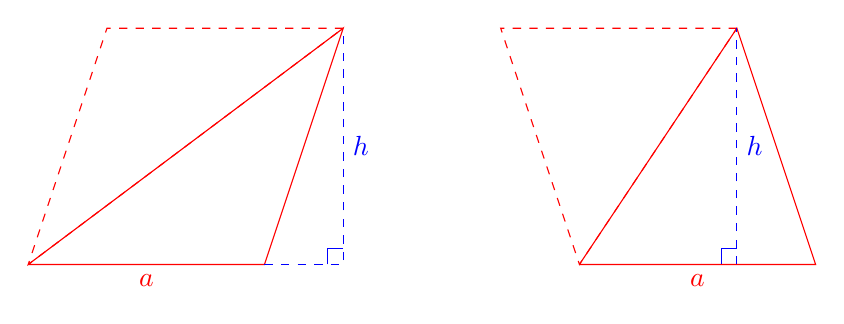
\begin{tikzpicture}
   \draw[color=red]
   (0,0) -- (1.5,0)node[below]{$a$} -- (3,0) -- (4,3) -- (0,0);

   \begin{scope}[rotate around={180:(2,1.5)}]
   \draw[color=red,dashed]
   (0,0) -- (1.5,0) -- (3,0) -- (4,3) -- (0,0);
   \end{scope}
   \draw[color=blue,dashed](3,0)--(4,0)--(4,1.5)node[right]{$h$}--(4,3);
   \draw[color=blue](3.8,0)--(3.8,.2)--(4,.2);

   \begin{scope}[shift={(7,0)}]
     \draw[color=red]
     (0,0) -- (1.5,0)node[below]{$a$} -- (3,0) -- (2,3) -- (0,0);
     \begin{scope}[rotate around={180:(1,1.5)}]
     \draw[color=red,dashed]
     (0,0) -- (3,0) -- (2,3) -- (0,0);
     \end{scope}
     \draw[color=blue,dashed](2,0)--(2,1.5)node[right]{$h$}--(2,3);
   \draw[color=blue](1.8,0)--(1.8,.2)--(2,.2);
   \end{scope}
 \end{tikzpicture}
\end{center}
\item Formule expressões da área para um triângulo rectângulo,
  isósceles rectângulo e equilátero.
 \end{enumerate}

\subsection*{Exercício 12 (polígonos regulares, Arquímedes)}

\begin{enumerate}
\item Utilize a régua e o compasso para construir: um círculo de centro $O$
  e raio $R$, o hexágono regular $ABCDEF$ de lado $R$ e inscrito en $C$,
  os raios ${OA}$, ${OB}$, \ldots, ${OF}$ e os seis apótemas do hexágono.
\item Expresse o perímetro, a longitude do apótema
   e a área do hexágono em função de $R$.
\item Consideremos o hexágono circunscrito a $C$, cujos apótemas
  são ${OA}$, ${OB}$, \ldots, ${OF}$. Qual é seu perímetro e
  área? Deduza uma aproximação do perímetro $P_C$ e área $A_C$ do círculo.
\item Suponhamos que o perímetro do círculo é proporcional a longitude do raio
  $P_C = 2 \pi R$. Indique uma aproximação da constante $\pi$.
\item De maneira geral, se considerarmos um polígono regular com $n \neq 6$
  lados de comprimento $l$ y apótema $h$, Quais são as fórmulas do perímetro e área?
\item Se tomarmos $n$ muito largo, o perímetro do $n$-ésimo polígono aproxima-se
  do perímetro de $P_C$, o apótema $h$ se aproxima do raio $R$ e
  a área do polígono aproxima-se da área $A_C$.
  Proponha uma fórmula para a área $A_C$ do círculo em função de $R,\pi$.
\end{enumerate}

\section{Volume do prisma}

De acordo com a Wikipédia, um prisma é todo poliedro formado por uma face
superior e uma face inferior paralelas e congruentes (também chamadas de bases)
ligadas por arestas. as Laterais de um prisma são quadriláteros ou paralelogramos.

\begin{center}
 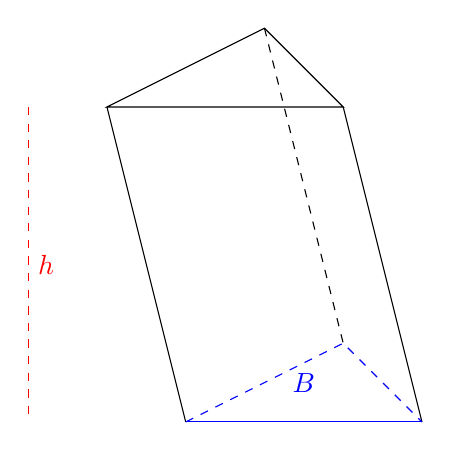
\begin{tikzpicture}
   \draw(0,4) -- (2,5) -- (3,4) --cycle (3,4) -- (4,0) (1,0) -- (0,4);
   \draw[blue] (1,0) -- (4,0);
   \draw[dashed] (2,5) -- (3,1);
   \draw[dashed,blue] (1,0) -- (3,1) -- (4,0);
   \draw[red,dashed] (-1,4) -- (-1,2)node[right]{$h$} -- (-1,0);
   \draw[blue](2.5,.5)node{$B$};
 \end{tikzpicture}
\end{center}

Se $B$ é a área da base e $h$ é a altura do prisma (distância entre suas bases),
o volume do prisma é $$V = B \times h$$

\subsection*{Exercício 13}

Determine o volume do prisma a seguir:

\begin{enumerate}
\item A base do prisma é um quadrado de lado $a=4\text{cm}$ e a altura
  do prisma é $h=3\text{cm}$
\item A base do prisma é um trapezoide de altura $h=2\text{cm}$ e bases de
  comprimento  $a=2\text{cm}$ e $b=4\text{cm}$ e a altura do prisma é
  $H=5\text{cm}$.
\item A base do prisma é um losango com diagonais medindo $p=3\text{cm}$ 
  e $q=4\text{cm}$ e a altura do prisma é $h = 8 \text{cm}$.
\item A base do prisma é um triangulo de base $b=\text{2}\text{cm}$ e
  altura $h=3\text{cm}$ e a altura do prisma é $H=7\text{cm}$.
\end{enumerate}

\subsection*{Exercício 14}

\begin{enumerate}
\item Considere o prisma de altura $h$ e cuja base é um hexagono inscrito em um
  circulo de raio $r$. Determine o volume do prisma.
\item Usando o exercício 12, desenvolva uma conjectura para o volume de um
  cilindro de altura $h$ e cuja base é um disco de raio $r$.
\end{enumerate}

\section{Soluções dos Exercícios}

\subsection*{Exercício 1}

Por exemplo, dois triângulos $ABC$ e $AEF$ retângulos em $A$ com
$1 = {AB} = {AC} = \frac{AE}{2} = \frac{AF}{2}$ possuem ângulos
$(90°, 45°, 45°)$ mais seus lados não são do mesmo tamanho.

A reciproca é impossível: se $ABC$ e $DEF$ são congruentes, temos
$\frac{DE}{AB} = \frac{EF}{BC} = \frac{FD}{CA} = 1$.

\subsection*{Exercício 2}

\begin{enumerate}
\item Temos
  $\widehat{C} = {180° - \widehat{A} - \widehat{B}} =
  {180° - \widehat{D} - \widehat{E}} = \widehat{F}$ e então
  os triângulos são semelhantes.
\item É fácil encontrar dois triângulos com $\widehat{A} = \widehat{D}$
  mas com outros ângulos não correspondentes.
\item Considere por exemplo $A = D$, $B = E$ e $AB = AC = DF$ mas
  $90° = \widehat{A} \neq \widehat{D} = 135°$.
\end{enumerate}

\subsection*{Exercício 3 (Tales)}

\begin{enumerate}
  \item São ângulos opostos pelo vértice.
  \item São ângulos alternados.
  \item São ângulos correspondentes.
\end{enumerate}

Desta igualdade de ângulos, vemos que $A_1B_1C_1$, $A_2B_2C_2$ e
$A_3B_3C_3$ são semelhantes a $ABC$.

\subsection*{Exercício 4 (pirâmide de Keops)}

Os raios do sol sã paralelos e portanto podemos mover a vara para que as
extremidades das sombras coincidam no mesmo ponto. Podemos aplicar o teorema de
Tales:
$$
\frac{B}{C} = \frac{A}{D}
$$
então $D = \frac{A C}{B} = \frac{1.63 \times
  \left(\frac{230}{2}+65\right)}{2} = 146.7m$

\subsection*{Exercício 5}

Traçando com a régua o eixo passando pelos pontos $(0,0)$ e $(1,0)$. Com o
compasso, podemos reportar o comprimento do segmento inicial sobre esse eixo
para obtermos os pontos $(2,0)$, $(3,0))$, \ldots que corresponde aos números
naturais.

O eixo ortogonal a mediatriz do segmento $[-1,1]$. O ponto $-1$ é construido da
mesma maneira que os números naturais. Com o compasso, traçamos os círculos de
centro $-1$ e $1$ e de raio $2$. Esses círculos se intersectam em dois pontos
sobre a mediatriz que podemos traçar utilizando a régua.

Com o compasso, retornamos retornamos ao segmento inicial para obtermos o ponto
$(0,1)$. Com a ŕegua, traçamos uma reta passando pelos pontos $(q,0)$ e $(0,1)$.

O círculo de centro $(p,0)$ e de raio $r=|p-q|$ corta a reta $D$ em
$Q_1={(q,0)}$ e outro ponto $Q_2$. Com a técnica acima, podemos traçar a
mediatriz de $[Q_1Q_2]$, que é a reta $D'$
ortogonal a $D$ passando por ${(p,0)}$. O círculo de raio $1$ e centro
$(p,0)$ corta essa recta $D'$ em dois pontos $P_1, P_2$. Novamente, traçando
a mediatriz de $[P_1P_2]$: é a reta passando por $(p,0)$ e paralela a
$D$, corresponde a reta azul.

A reta azul intersecta o eixo ortogonal no ponto
$(0,x)$ onde $x > 0$. Pelo teorema de Tales, obtemos
$$
x = \frac{x}{1} = \frac{p}{q}
$$

Com o compasso, podemos descobrir o comprimento $x$ sobre o eixo original para
obtermos o ponto $\left(\frac{p}{q}, 0 \right)$ correspondente a razão
$\frac{p}{q}$. Da mesma maneira, obtemos $-\frac{p}{q}$.
Os casos em que $p = 0$ e $p = q$ correspondem aos pontos originais  $0, 1$.
Então, podemos construir todos os números racionais.

\subsection*{Exercício 6}

\begin{enumerate}
\item $c = \sqrt{12^2 + 35^2} = 37$
\item $a = \sqrt{65^2 - 56^2} = 33$
\item $b = \sqrt{61^2 - 11^2} = 60$
\end{enumerate}

\subsection*{Exercício 7}

\begin{itemize}
  \item $A = c^2$
  \item $C = \left(a+b\right)^2 = a^2 + {2ab} + b^2$
  \item $B = 4 \times \frac{ab}{2} = {2ab}$
\end{itemize}

Então $a^2 + b^2 = C - B = A = c^2$.

\subsection*{Exercício 8 (construção da raiz quadrada)}

Traçamos uma reta com segmentos medindo $1$ e $x$ para obtermos um segmento de
comprimento $c = 1 + x$. Traçamos a mediatriz (ver exercício 5) deste segmento
para obtermos o centro do círculo vermelho que podemos desenhar com o compasso.
Utilizando a unidade de referência sobre o segmento obtemos os pontos de
coordenadas $0$ e $2$. A mediatriz do segmento formado por estes pontos
intersecta o círculo vermelho na nova longitude $h$.

Assim, as relações de Pitágoras são escritas como:
$$c^2 = a^2 + b^2,$$
$$a^2 = 1^2 + h^2,$$
$$b^2 = x^2 + h^2.$$

Então
${1^2+h^2 + x^2 + h^2} = a^2 + b^2 = c^2 = {(1+x)}^2 = 1^2+2x+x^2$,
$2h^2 = 2x$ e finalmente, $h = \sqrt{x}$.

\subsection*{Exercício 9}

$x = \frac{17}{3}$ é obtido utilizando a técnica do exercício 5.
$p = \sqrt{17}$, $q=\sqrt{3}$ e $\sqrt{x}$ são obtidos pela técnica do
exercício 8. Finalmente, $\frac{p}{q}$ é obtido como no exercício 5 (não precisa
que $p$ e $q$ sejam inteiros para fazer a construção). Podemos verificar que as
longitudes $\sqrt{x}$ e $\frac{p}{q}$ são iguais.

\subsection*{Exercício 7 (Quadriláteros)}

\begin{enumerate}
\item Um quadrado de lado $a$ possue perímetro $4a$ e área $a^2$. 
\item O perímetro do losango é $4c$ e
  sua área é a metade do retângulo azul, isso é $\frac{ab}{2}$.
\item A fórmula do perímetro é a mesma do retângulo: $2{(a+b)}$.
  Podemos cortar o triângulo rosa e mover parte dele para obtermos um
  retângulo de lados $a,h$ de mesma área: $a \times h$.
\item A área do trapezoide é metade do paralelogramo:
  $\frac{{(a+b)} \times h}{2}$.
\end{enumerate}

\subsection*{Exercício 8 (Triângulo)}

\begin{enumerate}
\item $a+b+c$
\item $3a$ (equilátero de lado $a$), $a+2b$ (isósceles de lado $a,b,b$)
  $a+b+\sqrt{a^2+b^2}$ (rectângulo de lados menores $a,b$),
  ${(2+\sqrt{2})}a$ (rectângulo isósceles de lados menor $a$).
\item É a metade do paralelogramo da figura: $\frac{a \times h}{2}$.
\item Um triângulo retângulo de lados menores $a,b$ (respectivamente
  rectângulo isósceles de lado menor $a$) é a metade de um retângulo de lado
  $a,b$ (respectivamente de um quadrado de lado $a$) y obtemos
  $\frac{ab}{2}$ e $\frac{a^2}{2}$. Na fórmula geral, $a$ é um lado menor
  e a altura $h$ é o outro lado menor.

  Para um triângulo equilátero de lado $a$, pelo Teorema de Pitágoras temos
  $h = \sqrt{a^2 - \left(\frac{a}{2}\right)^2} = \frac{\sqrt{3}}{2} a$ e
  então a área é $\frac{\sqrt{3}}{4} a^2$.
  
\end{enumerate}

\subsection*{Exercício 12 (polígonos regulares, Arquimedes)}

\begin{enumerate}
\item Obteremos:

\begin{center}
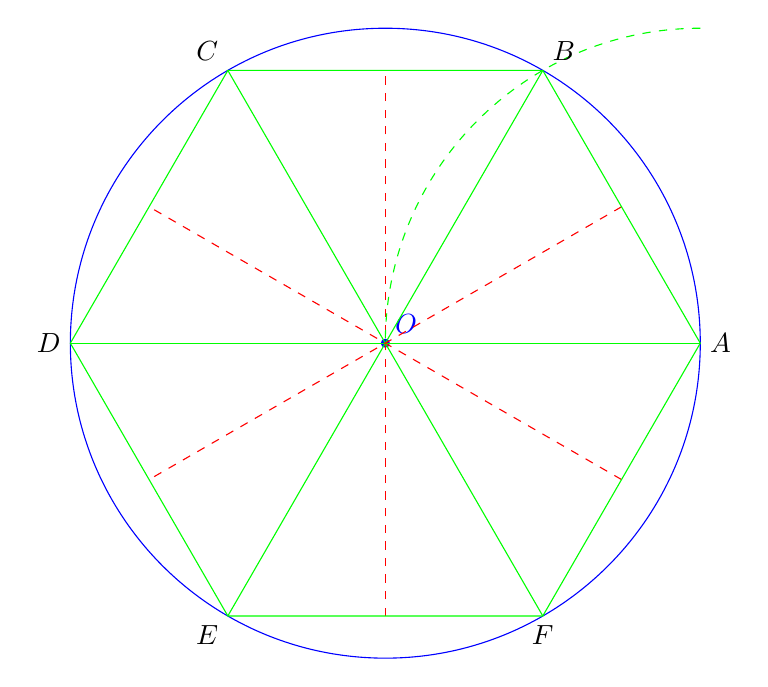
\begin{tikzpicture}
  \draw (0,0) circle(4)[color=blue];
  \draw[fill=black] (0,0) circle(.05)[color=blue] node[above right]{$O$};

  \draw (-4,0) -- (4,0)[color=green];
  \draw (0,-3.464101615137754) -- (0,3.464101615137754)[dashed,color=red];

  \begin{scope}[rotate around={60:(0,0)}]
  \draw (-4,0) -- (4,0)[color=green];
  \draw (0,-3.464101615137754) -- (0,3.464101615137754)[dashed,color=red];
  \end{scope}

  \begin{scope}[rotate around={120:(0,0)}]
  \draw (-4,0) -- (4,0)[color=green];
  \draw (0,-3.464101615137754) -- (0,3.464101615137754)[dashed,color=red];
  \end{scope}

  \draw (4,4) arc(90:180:4)[dashed,color=green];
  \draw (4,0) node[right]{$A$}
  -- (2,3.464101615137754)  node[above right]{$B$}
  -- (-2,3.464101615137754)  node[above left]{$C$}
  -- (-4,0)  node[left]{$D$}
  -- (-2,-3.464101615137754) node[below left]{$E$}
  -- (2,-3.464101615137754) node[below]{$F$}
  -- (4,0) [color=green];


\end{tikzpicture}
\end{center}

\item O hexágono possui $6$ lados de comprimento $R$ e então o
  perímetro é $6R$. Como no exercício 8, 
  a longitude do apótema é $\frac{\sqrt{3}}{2} R$ e 
  a área do hexágono é
  $6 \frac{\sqrt{3}}{4} R^2 = \frac{3 \sqrt{3}}{2} R^2$.
\item Esse é um hexágono de raio
  ${\frac{2}{\sqrt{3}} R}={\frac{2\sqrt{3}}{3} R}$ e então
  o perímetro é $4 \sqrt{3} R$ e área é $2 \sqrt{3} R^2$.
  Então $6R \leq P_C \leq 4 \sqrt{3} R$ e
  $\frac{3 \sqrt{3}}{2} R^2 \leq A_C \leq 2 \sqrt{3} R^2$.
\item $3 = \frac{6R}{2R} \leq \pi \leq \frac{4 \sqrt{3} R}{2R} = 2\sqrt{3} \approx 3.464101615137754$.
  Arquimedes utilizou $96$ polígonos para obter una melhor aproximação
  $3.1408 \approx \frac{310}{71} \leq \pi \leq \frac{31}{7} \approx 3.1429$.
\item Se o polígono possui $n$ lados de comprimento $l$, seu perímetro é $nl$.
  Sua área é composta de $n$ triângulos de lado $l$ e altura $h$ então
  é $n \frac{l \times h}{2} = \frac{nlh}{2}$.
\item O perímetro $nl$ se aproxima de $P_C = 2 \pi R$, a altura $h$ se aproxima
  de $R$. Então a área do polígono se aproxima de
  $\frac{2 \pi R \times R}{2} = \pi R^2$. De fato, podemos mostrar que
  a área de um círculo de raio $R$ é $A_C = \pi R^2$.
\end{enumerate}

\subsection*{Exercício 13}

\begin{enumerate}
\item $V = a^2 \times h = 48 \text{cm³}$.
\item $V = \frac{a+b}{2} \times h \times H = 30 \text{cm³}$
\item $V = \frac{p \times q}{2} \times h = 48 \text{cm³}$
\item $V=\frac{b \times h}{2} \times H = 21 \text{cm³}$
\end{enumerate}

\subsection*{Exercício 14}

\begin{enumerate}
\item Pelo exercício 12, a área dos hexágonos são $\frac{3 \sqrt{3}}{2} r^2$.
  Portanto o volume é $\frac{3 \sqrt{3}}{2} r^2 h$.
\item Considerando um prisma de altura $h$ e cuja base é um polígono regular
  inscrito em um círculo de raio $r$. Pelo exercício 12, quando aumentamos o
  número de lados na base a área aproxima-se de $\pi r^2$. O volume do prisma
  aproxima-se do volume de um cilindro, isso é $\pi r^2 h$.
\end{enumerate}
